\documentclass{article}

\usepackage[margin=1in]{geometry} 
\usepackage{amsmath,amsthm,amssymb,amsfonts, fancyhdr, color, comment, graphicx, environ, dsfont}

% \pagestyle{fancy}

\begin{document}

\section*{Famine of Forte}
This paper uses a search framework to prove several bounds concerning the proportion of good problems for a search algorithm. 

The paper uses a finite \textbf{search space} $\Omega$, and objective is to find an element of the \textbf{target set} $T \subset \Omega$. Given an order of the search space $\Omega$, we can represent $T$ as a binary vector of size $\Omega$, because each element of the search space corresponds to one index in our vector. This vector is the \textbf{target function}. 

Finally, the paper describes an information resource $F$. Similar to the No Free Lunch for Optimization paper, Famine of Forte treats $F$ as an oracle from which our algorithm gets all information about a particular point $\omega \in \Omega$. $F(\omega)$ is the evaluation of $\omega$. Interestingly, this paper abstracts this resource as a finite bit string. 

Given a search space $\Omega$, a target set $T$, and an information resource $F$, a search problem is defined as $(\Omega, F, T)$. Since we are abstracting $F$ and $T$ to be finite-length bit strings, we can do lots of fun things!

The paper describes a \textbf{Black-box Search Algorithm}, that attempts to find points $\omega$ in the target set $T$. The algorithm keeps track of its history $H$, which is a series of tuples $h_i = (\omega_i, F(\omega_i))$. Each tuple keeps track of the ith call to the oracle. At iteration $i$, the algorithm uses the history up to this point to compute a distribution $P_i$ over $\Omega$. The algorithm chooses some element $w_i$ according to the distribution and consults the oracle. Note especially that this algorithm will perform queries $i_{\text{max}}$ times - only after does it check if we have seen a target element.

\begin{center}
    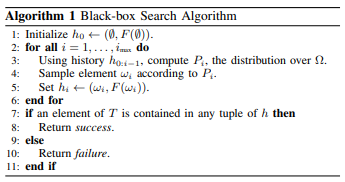
\includegraphics{BlackBoxAlgo.PNG}
\end{center}

We care about the performance of our search algorithm, since it is sufficiently general to represent many ML algorithms. 

Since the algorithm performs $i_{\text{max}}$ queries to the oracle, but this number can change, we may measure its performance by the expected per-query probability of success $q(T|F)$. The paper goes on to discuss how since this expectation is over all sources of randomness, it is equal to the probability of success for samples drawn from an appropriately averaged distribution - I don't really understand this. 

\begin{center}
    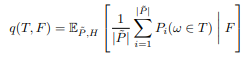
\includegraphics{ExpectedSuccess.PNG}
\end{center}

The paper defines $p(T,F)$ to be the expected probability of success when performing uniform random sampling, and uses this a baseline for the performance of our algorithm. It may be worth checking out the following paper, since it is referenced by Famine of Forte when discussion $p(T,F)$. 


W. Dembski and R. Marks II, “Conservation of information in search:
Measuring the cost of success,” Systems, Man and Cybernetics, Part A:
Systems and Humans, IEEE Transactions on, vol. 39, no. 5, pp. 1051
–1061, sept. 2009

\newpage

\textbf{Theorem 1.} Famine of Forte

This result shows that the proportion of search problems with performance $q(T,F) \geq q_{\text{min}}$ is bounded above. Formally, the paper defined a set $\tau_k$, which is a set of k-hot target vectors. That is, $\tau_k$ contains all possible k-element target sets. 

The paper restricts the potential information resources to be in the set $B_m$, where $B_m$ is any set of binary strings such that each string has length $m$ or less. The paper then defines sets $R$ and $R_{q_{min}}$, where $R$ contains all search problems with k-length target sets, and $R_{q_{min}}$ those problems that perform as well as $q_{min}$. Their definitions are below: 
\begin{align*}
    \tau_k &= \{T | T \subset Q, |T| = k \in \mathds{N}\} \\ 
    R &= \{(T,F) | T \in \tau_k, F \in B_m\} \\
    R_{q_{min}} &= \{(T,F) | T \in \tau_k, F \in B_m, q(T,F) \geq q_{min}\}
\end{align*}
Then 
\begin{align*}
    \frac{|R_{q_{min}}|}{|R|} \leq \frac{p}{q_{min}} = \frac{k / |\Omega|}{q_{min}}
\end{align*}
The same result holds as $m \to \infty$ - as the size of the information sets grows.

Essentially, we are given a search space $\Omega$. In that space, the proportion of problems $(\Omega, F, T)$ in which our algorithm performs as well as $q_{min}$ is bounded above by an exact quantity. 

\bigskip 

\textbf{Corollary 1.} (Conservation of Active Information of Expectations)

If we define $I_{q(T,F)} = - \log(p/q(T,F))$, and effectively use this metric as our performance (with minimum performance $b$), then we get the result 

\[\frac{|R_b|}{|R|} \leq 2^{-b}\]

This uses the exact same set construction as theorem 1. Note that $I_{q(T,F)}$ looks very similar to the difference in surprisals of $p$ and $q$ - $p$ and $q$ are expected per-query probabilities of success. Our algorithm does better than uniform random sampling if $I$ is large, since that indicates a higher per-query probability of success. Thus the proportion of problems that do as well as $b$ under this metric is bounded above by $2^{-b}$. The paper discusses how this shows that the improved search method is equivalent to a uniform random sampler on a reduced search space. (I'm not really sure how this works) 

\bigskip

\textbf{Theorem 2.} Famine of Favorable Strategies
\begin{center}
    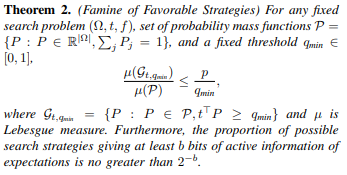
\includegraphics{FamineStrategy.PNG}
\end{center}

To be honest, I am not sure what this theorem is saying at the moment. My guess is that over all possible sequences $\{P_i\}_i$ of probabilities we can bound the number of algorithms that perform well on a given search problem. 

The paper discusses below how this places bounds on the number of favorable strategies on a given problem. This result and theorem 1 show that favorable problems for strategies and favorable strategies for problems are rare. 

\bigskip

\newpage
\textbf{Theorem 3.} Success Under Dependence
\begin{center}
    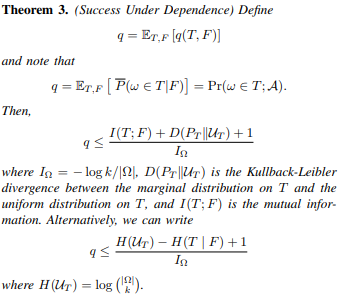
\includegraphics{SuccessUnderDependence.PNG}
\end{center}

This upper-bounds the expected performance of our algorithm on a search problem. The paper discusses how this bounds improves monotonically with the dependence between between our target set and information resources. That is, if our information is somewhat accurate, we can perform better! 

Other than that statement, I am having a hard time understanding this theorem. 


\bigskip

The paper then goes on to discuss examples of problems that fit under the framework, and proves theorem $1$ for the space of hyperparameters for a given algorithm $A$. It then shows that there cannot be a fitness function (information resource) that works well for all target sets in a search space. In other words, there is no One-Size-Fits-All fitness function. 

\bigskip

The paper then discusses why novel machine learning algorithms keep getting generated. Since the proportion of favorable strategies for a given problem is small and the proportion of favorable problems for a strategy is small, we must keep generating new strategies to deal with new problems.  

\subsubsection*{Further Reading} 

J. Culberson, “On the futility of blind search: An algorithmic view of
‘no free lunch’,” Evolutionary Computation, vol. 6, no. 2, pp. 109–127,
1998

** Just want to see no free lunch in another context

\bigskip

Compression and machine learning: a new perspective on feature space vectors

https://ieeexplore.ieee.org/abstract/document/1607268

** Compression - ML direction. 


\bigskip

An Introduction to Kolmogorov Complexity and Its Applications - skim chapters 2 and 3

** I read some stuff on Kolmogorov complexity, which is a way of measuring how random a string is / how hard a string is to generate. The complexity of a string is the number of characters needed to specify it (can use a programming language, so long as we include the specification in our length). Some strings are hard to generate, others are easy. There seems to already be a no-free-lunch theorem for compression based on the pigeonhold principle, but Kolmogorov complexity might help to give bounds on the number of strings that can be greatly compressed in a given language. 

\end{document}